\documentclass[nolayout]{article}

\usepackage[utf8]{inputenc}
\usepackage[english]{babel}
\usepackage{amsmath,amsthm}
\usepackage{geometry}
\usepackage{tikz}
\usetikzlibrary{fit,positioning}
\usepackage[textwidth=4cm,textsize=footnotesize]{todonotes}
\usepackage{fancyhdr}
\pagestyle{fancy}
\usepackage{amssymb,color,bbm,xargs}
\usepackage{graphicx}
\usepackage[active]{srcltx}
\usepackage{ifthen}
\usepackage{enumerate}
\usepackage{dsfont}
\usepackage{subcaption}

\newtheorem{lemma}{Lemma}
\newtheorem{proposition}{Proposition}
\newtheorem{theorem}{Theorem}
\newtheorem{corollary}{Corollary}

\definecolor{lavander}{cmyk}{0,0.48,0,0}
\definecolor{violet}{cmyk}{0.79,0.88,0,0}
\definecolor{burntorange}{cmyk}{0,0.52,1,0}
\definecolor{burntgreen}{cmyk}{0.62,0.44,0.47,0}
\definecolor{burntblue}{cmyk}{0.86,0.30,0.18,0}
\definecolor{palegreen}{cmyk}{0.86,0.30,0.96,0}


\def\sup{\mathrm{sup}}
\def\param{\theta}
\def\paramset{\Theta}
\def\1{\mathds{1}}
\def\rset{\mathbb{R}}
\def\rmd{\mathrm{d}}
\def\eqsp{\,}
\def\Pstar{\mathbb{P}_{\pi_{\star}}}
\def\bayes{\pi_{\star}}
\def\kernel{\mathsf{M}}
\newcommand{\limit}[1]{\underset{#1\to \infty}{\longrightarrow}}
\newcommand{\E}{\mathbb{E}}
\newcommand{\kullback}{\mathsf{L}}
\newcommand{\link}{\leftrightarrow}


\newcommand{\pa}[1]{\left(#1\right)}
\newcommand{\cro}[1]{\left[#1\right]}
\newcommand{\set}[1]{\left\{#1\right\}}
\newcommand{\PE}[1]{\left\lfloor#1\right\rfloor}

\newcommand{\loss}[1]{\ell\pa{#1}}
\newcommand{\Lo}[2]{\ell^{#1}\pa{#2}}

\newcommand{\bN}{\mathbb{N}}
\newcommand{\bP}{\mathbb{P}}
\newcommand{\bR}{\mathbb{R}}
\newcommand{\bZ}{\mathbb{Z}}

\newcommand{\cA}{\mathcal{A}}
\newcommand{\cD}{\mathcal{D}}
\newcommand{\cE}{\mathcal{E}}
\newcommand{\cO}{\mathcal{O}}
\newcommand{\cS}{\mathcal{S}}
\newcommand{\cV}{\mathcal{V}}
\newcommand{\cX}{\mathcal{X}}

\newcommand{\ordermax}[2]{{\mathsf{q}}^{#1}_{#2}}
\newcommand{\remainder}[2]{{\mathsf{r}}^{#1}_{#2}}

\newcommand{\condlik}{k}
\newcommand{\card}{\mathrm{card}}

\newcommand{\MLE}{\widehat{\pi}}

\newcounter{hypH}
\newenvironment{hypH}{\refstepcounter{hypH}\begin{itemize}
\item[{\bf H\arabic{hypH}}]}{\end{itemize}}
\begin{document}

\title{Early learning in Bradley-Terry tournaments}
\date{}

\author{}

\lhead{}
\rhead{MLE for the Bradley-Terry tournaments in random environment}

\maketitle

\begin{abstract}

\end{abstract}
\section{Setting}
\subsection{Bradley-Terry tournament (BTT) in random environment}
Consider a tournament involving an even number $N$ of players called $[N]=\{1,\ldots,N\}$. During the tournament, players face each other at most once. When $i$ faces $j$, the result is the victory of either $i$ or $j$, we call $X_{i,j}=1$ if $i$ beats $j$ and $X_{i,j}=0$ if $j$ beats $i$, in particular $X_{i,j}=1-X_{j,i}$. Every player $i$ has a value $v_i>0$ and this value is used to compute the probabilities
\[
\bP(X_{i,j}=1|v_i,v_j)=\frac{v_i}{v_i+v_j}\enspace.
\]
Moreover, given $v=(v_i)_{i\in[N]}$ the r.v. $(X_{i,j})_{1\le i<j\le N}$ are assumed independent. To ease notation, for every vector $a\in \bR^p$ and every subset $B\subset [p]=\{1,\ldots,p\}$, we denote by $a_{B}=\{a_i,\;i\in B\}$. Define, for all $x\in \{0,1\}$ and all $(v_1,v_2)\in(\bR_+^*)^2$, 
\[
\condlik(x,v_{[2]})=\frac{v_1^xv_2^{1-x}}{v_1+v_2}\enspace,
\]
so that $\bP(X_{i,j}=x|v_{\{i,j\}})=k(x,v_{\{i,j\}})$. In our model, $v=(v_i)_{i\in [N]}$ is a vector in $\bR^N$ with i.i.d. entries with common unknown distribution $\bayes$ that is set once and for all before the tournament begins. 

A voir
\begin{enumerate}
 \item Loi quenched et annealed?
\end{enumerate}

\subsection{Round-robin days in BTT and early learning task}
In this paper, we do not assume that all the pairs meet once and we describe in this section the round-robin algorithm that gives at each time $t\in[N]$ the pairs that face each others. At time $t=1$, the players are disposed according to Figure~\ref{fig:robin:day1}. Each player faces the one in front of him, that is $2i-1$ faces $2i$, for all $i\in[N/2]$. 
\begin{figure}
\centering
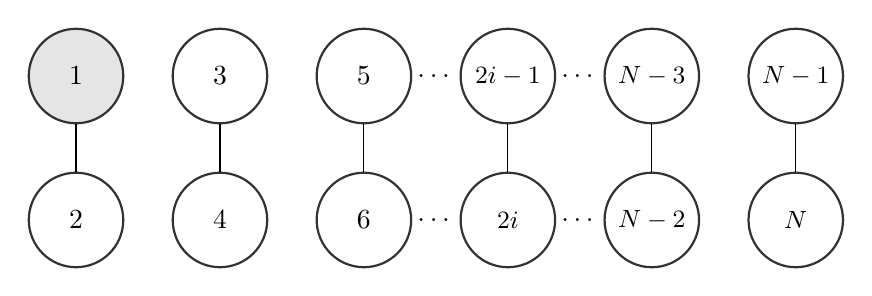
\begin{tikzpicture}
\tikzstyle{main}=[circle, minimum size = 12mm, thick, draw =black!80, node distance = 6mm]
\tikzstyle{connect}=[-latex, thick]
\tikzstyle{box}=[rectangle, draw=black!100]
\node[main, fill = black!10] (v1){$1$ };
\node[main] (v3) [right=of v1] {$3$ };
\node[main] (v5) [right=of v3] {$5$ };
\node[main] (v7) [right=of v5] {{\small$2i-1$}};
\node[main] (v9) [right=of v7] {{\small$N-3$}};
\node[main] (v11) [right=of v9] {{\small$N-1$}};
\node[main] (v2) [below=of v1] {$2$};
\node[main] (v4) [below=of v3] {$4$};
\node[main] (v6) [below=of v5] {$6$};
\node[main] (v8) [below=of v7] {{\small$2i$}};
\node[main] (v10) [below=of v9] {{\small$N-2$}};
\node[main] (v12) [below=of v11] {{\small$N$}};
\draw (v1) -- (v2);
\draw (v3) -- (v4);
\draw (v5) -- (v6);
\draw (v7) -- (v8);
\draw (v9) -- (v10);  
\draw (v11) -- (v12);     
\path (v5) -- node[auto=false]{\ldots}  (v7); 
\path (v7) -- node[auto=false]{\ldots}  (v9); 
\path (v6) -- node[auto=false]{\ldots}  (v8); 
\path (v8) -- node[auto=false]{\ldots}  (v10);    
\end{tikzpicture}
\caption{Round-robin, day $1$.}
\label{fig:robin:day1}
\end{figure}
At time $t=2$, the disposition of the players changes according to the round-robin algorithm described in Figure~\ref{fig:robin:day2}. Player $1$ does not move, $2$ takes the place of $3$, each odd integer $2i-1<N-1$ takes the place of $2i+1$, $N-1$ takes the place of $N$ and each even integer $2i>2$ takes the place of $2(i-1)$. Once they moved, each player faces the opponent in front of him.
\begin{figure}
\centering
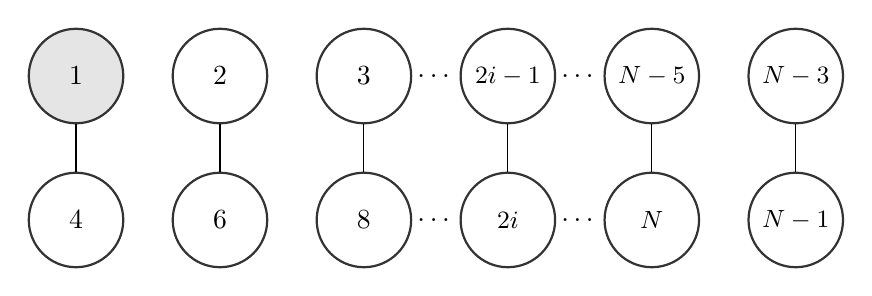
\begin{tikzpicture}
\tikzstyle{main}=[circle, minimum size = 12mm, thick, draw =black!80, node distance = 6mm]
\tikzstyle{connect}=[-latex, thick]
\tikzstyle{box}=[rectangle, draw=black!100]
\node[main, fill = black!10] (v1){$1$ };
\node[main] (v3) [right=of v1] {$2$ };
\node[main] (v5) [right=of v3] {$3$ };
\node[main] (v7) [right=of v5] {{\small$2i-1$}};
\node[main] (v9) [right=of v7] {{\small$N-5$}};
\node[main] (v11) [right=of v9] {{\small$N-3$}};
\node[main] (v2) [below=of v1] {$4$};
\node[main] (v4) [below=of v3] {$6$};
\node[main] (v6) [below=of v5] {$8$};
\node[main] (v8) [below=of v7] {{\small$2i$}};
\node[main] (v10) [below=of v9] {{\small$N$}};
\node[main] (v12) [below=of v11] {{\small$N-1$}};
\draw (v1) -- (v2);
\draw (v3) -- (v4);
\draw (v5) -- (v6);
\draw (v7) -- (v8);
\draw (v9) -- (v10);   
\draw (v11) -- (v12);     
\path (v5) -- node[auto=false]{\ldots}  (v7); 
\path (v7) -- node[auto=false]{\ldots}  (v9); 
\path (v6) -- node[auto=false]{\ldots}  (v8); 
\path (v8) -- node[auto=false]{\ldots}  (v10);   
\end{tikzpicture}
\caption{Round-robin, day $2$.}
\label{fig:robin:day2}
\end{figure}

At time $t\ge 2$, each player moves once according to the round-robin algorithm and plays the opponent in front of him. Each time $t\in\bN$ is called a day of the tournament. It is well known that, at day $N$, all players have faced each other once. 

In this paper, we assume that the results of all games up to day $n$ are available and we want to infer the distribution $\bayes$ from this data set. The time $n$ is assumed to be much smaller than $N$ and this is why we called this problem the ``early learning task". The set of couples $(i,j)\in[N]^2$, with $i<j$ such that $i$ has played $j$ before time $n$ is denoted by $\cA_{n,N}$, in other words, the data set is $\cD_{n,N}=\{(X_{i,j})_{(i,j)\in A_{n,N}}\}$.


\subsection{Estimation of the environment distribution}
Our estimation strategy is quite standard. Let $\Pi$ denote a set of densities $\pi$ on $\bR_+^*$. For technical reasons, every $\pi\in\Pi$ assumed to be supported in $[\epsilon,1]$ for some $\epsilon>0$. The log-likelihood of the observations is defined, for all $\pi\in\Pi$, by:
\[
\Lo{\cD_{n,N}}{\pi}:=-\log\cro{\int  \pa{\prod_{(i,j)\in A_{n,N}}k(X_{i,j},v_{\{i,j\}})}\pi^{\otimes N}(dv)}\enspace.
\]
Our estimator is then any maximum likelihood estimator (MLE):
\[
\MLE\in \arg\min_{\pi\in\Pi}\Lo{\cD_{n,N}}{\pi}\enspace.
\]
We shall often forget the dependence of the log-likelihood in the data set $\cD_{n,N}$ and write $\loss{\pi}=\Lo{\cD_{n,N}}{\pi}$.

\begin{enumerate}
\item On pourrait supposer que toutes les lois sont a support dans un meme compact plutot que dans $[\epsilon,1]$, c'est equivalent par invariance par changement d'echelle.
\end{enumerate}

\section{Loss of memory properties in the early learning problem}

In this section, we assume that $N\to\infty$ and $n\ll N$.

\subsection{Graphical model of the round-robin BTT}
The purpose of this section is to build a graph representing the conditional dependences between the variables $v$ and $X=(X_{i,j})_{(i,j)\in A_{n,N}}$. This graph is directed and is denoted $G^{(n,N)}=(V^{(n,N)},E^{(n,N)})$. The set of vertices is a disjoint union $V^{(n,N)}=V^{(n,N)}_{p}\cup V^{(n,N)}_g$ where $V^{(n,N)}_p$ is a partition of $[N]$ and $V^{(n,N)}_g$ is a partition of $ A_{n,N}$. 

Start with the undirected graph $(V^{(n,N)}_0,E^{(n,N)}_0)$ where $V^{(n,N)}_0=[N]$ and $E^{(n,N)}_0=\{\{i,j\} : (i,j)\in A_{n,N}\}$, that is the graph where the nodes are the players and an edge is drawn between players who play together. The graph $(V^{(n,N)}_0,E^{(n,N)}_0)$ is endowed with the graph distance $d^{(n,N)}_0$, that is $d^{(n,N)}_0(i,j)$ is the minimal length of a path between the nodes $i$ and $j$ in $V^{(n,N)}_0$. One can write $[N]=\{1\}\cup\cup_{q=1}^{N}V^{(n,N)}_{p,q}$, where, for any $q\in[N]$, $V^{(n,N)}_{p,q}$ is the set of $i\in[N]$ such that $d^{(n,N)}_0(1,i)=q$. Figure~\ref{fig:robin:partitionP} displays this partition for $n = 3$.

\begin{figure}
\centering
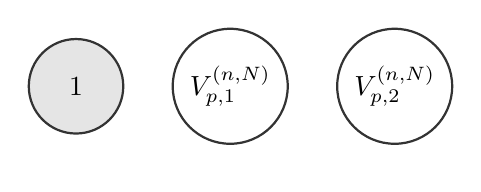
\begin{tikzpicture}
\tikzstyle{main}=[circle, minimum size = 12mm, thick, draw =black!80, node distance = 6mm]
\tikzstyle{connect}=[-latex, thick]
\tikzstyle{box}=[rectangle, draw=black!100]
\node[main, fill = black!10] (v1){$1$ };
\node[main,label=below:] (v2) [right=of v1] {$V^{(n,N)}_{p,1}$}; 
\node[main,label=below:] (v3) [right=of v2] {$V^{(n,N)}_{p,2}$ }; 
\end{tikzpicture}
\caption{Round-robin, partition of $[N]$, $n=3$.}
\label{fig:robin:partitionP}
\end{figure}


Let $(\cE,\cO)$ denotes the following partition of $[N]$. $\cE$ contains all $i$ that play $1$ an even day before time $N/2$ (i.e. the set $\cE_1$ of all $i$ such that $\{1,i\}\in A_{N/2,N}$) and their opponent at time $1$ (i.e. the set $\cE_2$ of all $i$ such that $\{i,j\}\in A_{1,N}$, for some $j\in \cE_1$), $\cO$ contains $1$ and all $i$ that play $1$ an odd day before time $N/2$. For any $q\ge 1$, let $V^{(n,N)}_{p,q,e}=V^{(n,N)}_{p,q}\cap \cE$ and $V^{(n,N)}_{p,q,o}=V^{(n,N)}_{p,q}\cap \cO$. The vertices $V_p^{(n,N)}=\{\{1\},(V^{(n,N)}_{p,q,e},V^{(n,N)}_{p,q,o})_{q\in[N]}\}$, the empty elements in this collection can be dropped off. These partitions can be visualized in the following picture.

 

The round-robin algorithm induces an important property that we will now use to derive from this first partition the partition $V_g$. Call $i$ the player in position $i$ on figure~\ref{fig:robin:day1}.

\begin{proposition}\label{prop:RRProp}
Let $1<t\le N/4-1$. If $t$ is odd, at time $t$, every $i\notin \{N,N-2x+1, x=0,\ldots,2t\}$, that is every $i$ that did not play $N-1$ before time $t$ nor $N$ before time $t-1$, plays a $j$ in the same element in the partition $(\cE,\cO)$, that is $i\in \cE$ plays a $j\in\cE$ and every $i\in \cO$ plays a $j\in\cO$. if $t$ is even, $i\notin \{N,N-2x+1, x=1,\ldots,2t\}$ plays either $1$ or a $j$ in the same element of the partition $(\cE,\cO)$.  
\end{proposition}

Proposition~\ref{prop:RRProp} can easily be checked by induction. It implies the following corollary that we'll use to build the partition of $X$.

\begin{corollary}
Let $u\in\{e,o\}$. For any $n<N/2$, any $q$ such that $N-1\notin V_{p,q,u}\cup V_{p,q+1,u}$ and any $i\in V^{(n,N)}_{p,q,u}$, any $j$ such that $\{i,j\}\in A_{n,N}$ belongs to the union $V^{(n,N)}_{p,q-1,u}\cup V^{(n,N)}_{p,q,u}\cup V^{(n,N)}_{p,q+1,u}$, with the convention that $V^{(n,N)}_{p,0,u}=\{1\}$.
\end{corollary}
\begin{proof}
 Fix $n$, $q\in[1,q_u-1]$, $i\in V_{p,q,u}^{(n,N)}$ and let $j$ such that $\{i,j\}\in A_{n,N}$. By definition $d_0^{(n,N)}(1,i)$ and $d_0^{(n,N)}(i,j)=1$, thus by the triangular inequality
 \[
q-1= d^{(n,N)}_0(1,i)-d^{(n,N)}_0(i,j)\le d^{(n,N)}_0(1,j)\le d^{(n,N)}_0(1,i)+d^{(n,N)}_0(i,j)=q+1\enspace.
 \]
 Therefore, $j\in V^{(n,N)}_{p,q-1}\cup V^{(n,N)}_{p,q}\cup V^{(n,N)}_{p,q+1}$. Moreover, $i$ cannot play $N-1$ nor $N$, therefore, by Proposition~\ref{prop:RRProp}, either $j=1$, which is only possible if $q=1$ or $i$ and $j$ belong to the same element of the partition $(\cE,\cO)$.
\end{proof}

\subsection{Bounding the kernel}
%The loglikelihood of the observations may be decomposed as:
%\begin{align*}
%\Lo{\cD_{n,N}}{\pi} &= \log \left(p^{\pi}_{\cD_{n,N}}(X)\right)\eqsp,\\
%&= \log\left(p^{\pi}_{\cD_{n,N}}\left(V^{(n,N)}_{p,f}\right)\right) +  \log\left(p^{\pi}_{\cD_{n,N}}\left(V^{(n,N)}_{p,\cdot,e}\middle|V^{(n,N)}_{p,f}\right)\right) + \log\left(p^{\pi}_{\cD_{n,N}}\left(V^{(n,N)}_{p,\cdot,o}\middle|V^{(n,N)}_{p,\cdot,e}\eqsp,V^{(n,N)}_{p,f}\right)\right) \eqsp.
%\end{align*}
%First note that:
%\[
%\log\left(p^{\pi}_{\cD_{n,N}}\left(V^{(n,N)}_{p,\cdot,e}\middle|V^{(n,N)}_{p,f}\right)\right) = \log\left(p^{\pi}_{\cD_{n,N}}\left(V^{(n,N)}_{p,\bar q,e}\middle|V^{(n,N)}_{p,f}\right)\right) + \sum_{q=1}^{\bar q -1}\log\left(p^{\pi}_{\cD_{n,N}}\left(V^{(n,N)}_{p,q,e}\middle|V^{(n,N)}_{p,[q+1,\bar q],e},V^{(n,N)}_{p,f}\right)\right)
%\]


\section*{Bradley-Terry model in the case $n=2$}
Let $N$ be the number of players and $(v_i)_{1\le i\le N}$ be the scores associated with each player. It is assumed that the $(v_i)_{1\le i\le N}$ are i.i.d. and that the distribution of $v_1$ has probability density function $\pi_{\param}$ on $C_{\param}\subset \rset_+^{\star}$ with respect to a reference measure $\mu$. Conditional on $(v_i)_{1 \le i \le N}$, the observations $(X_{1,2},X_{1,3}, X_{2k-2,2k}, X_{2k-1,2k+1})_{2\le k \le (N-1)/2}$ are independent and, for each $1\le \ell\le N-2$, the conditional distribution of $X_{\ell,\ell+2}$ given $(v_i)_{1\le i\le N}$ has probability density function:
\begin{equation}
\label{eq:defG}
x\mapsto G (x;v_{\ell},v_{\ell+2}) = \frac{v_{\ell}^x\,v_{\ell+2}^{1-x}}{v_{\ell} + v_{\ell+2}}
\end{equation}
with respect to the counting measure. The conditional distribution of $X_{1,2}$ given $(v_i)_{1\le i\le N}$ has probability density function $x\mapsto G (x;v_{1},v_{2})$ with respect to the counting measure.
The graphical model associated with Bradley-Terry model in the case $n=2$ is displayed in Figure~\ref{fig:bt}.
\begin{figure}[h!]
\centering
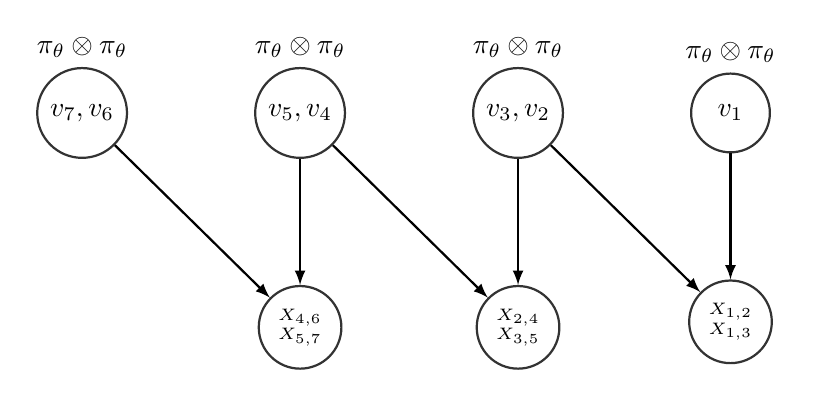
\begin{tikzpicture}
\tikzstyle{main}=[circle, minimum size = 10mm, thick, draw =black!80, node distance = 16mm]
\tikzstyle{connect}=[-latex, thick]
\tikzstyle{box}=[rectangle, draw=black!100]
  \node[main,label=above:$\pi_{\param}\otimes\pi_{\param}$] (v4) {$v_{7}, v_{6}$};
  \node[main,label=above:$\pi_{\param}\otimes\pi_{\param}$] (v3) [right=of v4] {$v_5, v_4$};
  \node[main,label=above:$\pi_{\param}\otimes\pi_{\param}$] (v2) [right=of v3] {$v_3, v_2$};
  \node[main,label=above:$\pi_{\param}\otimes\pi_{\param}$] (v1) [right=of v2] {$v_1$};
  \node[main] (X3) [below=of v3] {{\small $\substack{X_{4,6}\\ X_{5,7}}$}};
  \node[main] (X2) [below=of v2] {{\small $\substack{X_{2,4}\\ X_{3,5}}$}};
  \node[main] (X1) [below=of v1] {{\small $\substack{X_{1,2}\\ X_{1,3}}$}};
  \path (v1) edge [connect] (X1)
           (v2) edge [connect] (X1)
           (v2) edge [connect] (X2)
	   (v3) edge [connect] (X2)
           (v3) edge [connect] (X3)
           (v4) edge [connect] (X3);
\end{tikzpicture}
\caption{Bradley-Terry graphical model in the case $n=2$ and $N=7$.}
\label{fig:bt}
\end{figure}

Consider the following assumptions on the model.

\begin{hypH}
\label{assum:strongmix}
There exist $0<\sigma_-<\sigma_+<\infty$ such that for all $\param\in\param$ and all $v\in C_{\param}$, $\sigma_-\le \pi_{\param}(v)\le\sigma_+$.
\end{hypH}

\begin{hypH}
\label{assum:compact}
There exist $0<c_-<c_+<\infty$ such that for all $\param\in\param$, $C_{\param} \subset (c_-,c_+)$.
\end{hypH}

Define 
\begin{equation}
\label{eq:def:rho}
\rho = 1- \left(\frac{c_-\sigma_-}{(c_-+c_+)\sigma_+}\right)^2\eqsp.
\end{equation}

Define $\bar C_{\param} = C_{\param}\times C_{\param}$, $\bar v_1 = v_1$, $\bar X_1 = (X_{1,2},X_{1,3})$ and for all $k\ge 2$, $\bar v_k = (v_{2k-2},v_{2k-1})$ and $\bar X_k = (X_{2k-2,2k},X_{2k-1,2k+1})$. Conditional on $(\bar v_i)_{i\ge 1}$, the observations $(\bar X_i)_{i\ge 1}$ are independent and, for each $\ell\ge 1$ the conditional distribution of $\bar X_{\ell}$ given $(\bar v_i)_{i\ge 1}$ has probability density function:
\[
\bar x = (x_1,x_2) \mapsto \bar G (\bar x;\bar v_{\ell+1},\bar v_{\ell}) = G (x_1,v_{2\ell},v_{2\ell+2})G (x_2;v_{2\ell-1},v_{2\ell+1})\eqsp,
\]
where $G$ is defined by \eqref{eq:defG}.
\begin{figure}
\label{fig:bt:extended}
\centering
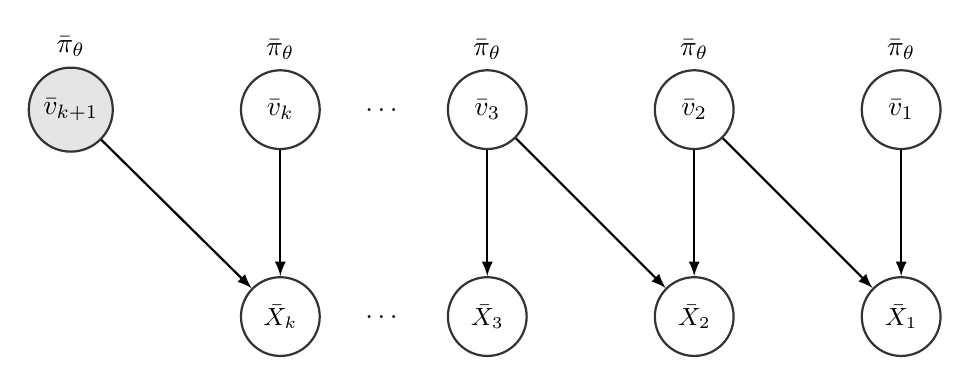
\begin{tikzpicture}
\tikzstyle{main}=[circle, minimum size = 10mm, thick, draw =black!80, node distance = 16mm]
\tikzstyle{connect}=[-latex, thick]
\tikzstyle{box}=[rectangle, draw=black!100]
  \node[main, fill = black!10,label=above:$\bar \pi_{\param}$] (v5){$\bar v_{k+1}$ };
  \node[main,label=above:$\bar \pi_{\param}$] (v4) [right=of v5] {$\bar v_{k}$ };
  \node[main,label=above:$\bar \pi_{\param}$] (v3) [right=of v4] {$\bar v_3$};
  \node[main,label=above:$\bar \pi_{\param}$] (v2) [right=of v3] {$\bar v_2$};
  \node[main,label=above:$\bar \pi_{\param}$] (v1) [right=of v2] {$\bar v_1$};
  \node[main] (X4) [below=of v4] {{\small $\bar X_{k}$}};
  \node[main] (X3) [below=of v3] {{\small $\bar X_{3}$}};
  \node[main] (X2) [below=of v2] {{\small $\bar X_{2}$}};
  \node[main] (X1) [below=of v1] {{\small $\bar X_{1}$}};
  \path (v1) edge [connect] (X1)
           (v2) edge [connect] (X1)
           (v2) edge [connect] (X2)
	   (v3) edge [connect] (X2)
           (v3) edge [connect] (X3)
           (v5) edge [connect] (X4)
           (v4) edge [connect] (X4);
  \path (v4) -- node[auto=false]{\ldots}  (v3);  
  \path (X4) -- node[auto=false]{\ldots} (X3);        
\end{tikzpicture}
\caption{Bradley-Terry graphical model in the case $n=2$ with extended states.}
\end{figure}

\subsection*{Forgetting properties of the Bradley-Terry model}
For all $1\le k < n$ and all probability density function $\lambda$ on $\bar C_{\param}$, denote by $\phi^{n,k}_{\lambda,\param}$ the probability density of the conditional distribution of $\bar v_k$ given $(\bar X_n,\ldots,\bar X_k)$ when the state $\bar v_{n+1}$ has probability density function $\lambda$ on $\bar C_{\param}$. Note that for all $1\le k \le n < m$,
\begin{align*}
\phi^{m,k}_{\lambda,\param}\left(\bar v_{k}\right) &= \frac{\int \lambda(\bar v_{m+1})\prod_{i = m}^k\bar G(\bar X_i; \bar v_{i+1},\bar v_i) \bar \pi_{\param}(\bar v_i)\mu(\rmd \bar v_{m+1:k+1})}{\int \lambda(\bar v_{m+1})\prod_{i = m}^k\bar G(\bar X_i; \bar v_{i+1},\bar v_i) \bar \pi_{\param}(\bar v_i)\mu(\rmd \bar v_{m+1:k})} = \phi^{n,k}_{\eta^{m,n}_{\lambda,\param},\param}\left(\bar v_{k}\right)\eqsp,
\end{align*}
where, $\eta^{m,n}_{\lambda,\param}$ is the probability density function defined on $\bar C_{\param}$ as:
\[
\eta^{m,n}_{\lambda,\param}: \bar v_{n+1} \mapsto \frac{\int \lambda(\bar v_{m+1})\bar G(\bar X_m; \bar v_{m+1},\bar v_m)\prod_{i = m}^{n+2} \bar \pi_{\param}(\bar v_i) \bar G(\bar X_{i-1}; \bar v_{i},\bar v_{i-1}) \mu(\rmd \bar v_{m+1:n+2})}{\int \lambda(\bar v_{m+1})\bar G(\bar X_m; \bar v_{m+1},\bar v_m)\prod_{i = m}^{n+2} \bar \pi_{\param}(\bar v_i) \bar G(\bar X_{i-1}; \bar v_{i},\bar v_{i-1}) \mu(\rmd \bar v_{m+1:n+1})}\eqsp.
\]
For all $n\ge1$, and all $\param\in\param$, the likelihood of the observations is given by:
\[
L^n_{\pi_{\param},\param}\left(\bar X_{1},\ldots,\bar X_{n}\right) = p_{\pi_{\param},\param}\left(\bar X_n\right)\prod_{k=1}^{n-1}p_{\pi_{\param},\param}\left(\bar X_{k}\middle| \bar X_{n},\ldots,\bar X_{k+1}\right)
\] 
and the loglikelihood is written:
\[
\ell^n_{\pi_{\param},\param}\left(\bar X_{1},\ldots,\bar X_{n}\right) = \log L^n_{\pi_{\param},\param}\left(\bar X_{1},\ldots,\bar X_{n}\right) = \log p_{\pi_{\param},\param}\left(\bar X_n\right) + \sum_{k=1}^{n-1}\log p_{\pi_{\param},\param}\left(\bar X_{k}\middle| \bar X_{n},\ldots,\bar X_{k+1}\right)\eqsp.
\]
For all $2\le k\le n <m$,
\begin{equation}
\label{eq:incremental:likelihood}
p_{\pi_{\param},\param}\left(\bar X_{k}\middle| \bar X_{n},\ldots,\bar X_{k+1}\right) = \int_{\bar C_{\param}^2}\phi^{n,k+1}_{\pi_{\param},\param}\left(\bar v_{k+1}\right)\pi_{\param}(\bar v_{k})\bar G(\bar X_{k};\bar v_{k+1},\bar v_{k})\mu(\rmd \bar v_{k:k+1})
\end{equation}
and 
\begin{align*}
p_{\pi_{\param},\param}\left(\bar X_{k}\middle| \bar X_{m},\ldots,\bar X_{k+1}\right) &= \int_{\bar C_{\param}^2}\phi^{m,k+1}_{\pi_{\param},\param}\left(\bar v_{k+1}\right)\pi_{\param}(\bar v_{k})\bar G(\bar X_{k};\bar v_{k+1},\bar v_{k})\mu(\rmd \bar v_{k:k+1})\eqsp,\\
&=\int_{\bar C_{\param}^2}\phi^{n,k+1}_{\eta^{m,n}_{\pi_{\param},\param},\param}\left(\bar v_{k+1}\right)\pi_{\param}(\bar v_{k})\bar G(\bar X_{k};\bar v_{k+1},\bar v_{k})\mu(\rmd \bar v_{k:k+1})\eqsp.
\end{align*}
\begin{lemma}
\label{lem:uniformforgetting}
Assume that H\ref{assum:strongmix} and H\ref{assum:compact} hold. Then, for all $1\le k \le n < m$, $\Pstar$-a.s.,
\[
\sup_{\param\in\paramset}\left|\log p_{\pi_{\param},\param}\left(\bar X_{k}\middle| \bar X_{n},\ldots,\bar X_{k+1}\right) - \log p_{\pi_{\param},\param}\left(\bar X_{k}\middle| \bar X_{m},\ldots,\bar X_{k+1}\right)\right| \le \left(1+\frac{c_+}{c_-}\right)^2\rho^{n-k}\eqsp,
\]
where $\rho$ is defined by \eqref{eq:def:rho}.
In addition,
\[
\sup_{\param\in\paramset;\;n\ge k}\left|\log p_{\pi_{\param},\param}\left(\bar X_{k}\middle| \bar X_{n},\ldots,\bar X_{k+1}\right)\right|\le 2\log\left(1+\frac{c_+}{c_-}\right)\eqsp. 
\]
\end{lemma}
\begin{proof}
To prove the first inequality, note that
\begin{multline}
\left|p_{\pi_{\param},\param}\left(\bar X_{k}\middle| \bar X_{n},\ldots,\bar X_{k+1}\right) - p_{\pi_{\param},\param}\left(\bar X_{k}\middle| \bar X_{m},\ldots,\bar X_{k+1}\right)\right|\\
= \left|\left(\phi^{n,k+1}_{\eta^{m,n}_{\pi_{\param},\param},\param} - \phi^{n,k+1}_{\pi_{\param},\param}\right)\left[\int_{\bar C_{\param}}\pi_{\param}(\bar v_{k})\bar G(\bar X_{k};\cdot,\bar v_{k})\mu(\rmd \bar v_{k})\right]\right|\eqsp.\label{eq:diff:likelihood}
\end{multline}
Conditional on $(\bar X_n,\ldots,\bar X_{k+1})$, $(\bar v_{n+1},\ldots,\bar v_{k+1})$ is a Markov chain with kernel:
\begin{align*}
p_{\param}\left(\bar v_{p}\middle | \bar v_{n+1},\ldots, \bar v_{p+1},\bar X_n,\ldots,\bar X_{k+1}\right) &=  p_{\param}\left(\bar v_{p}\middle |\bar v_{p+1},\bar X_p,\ldots,\bar X_{k+1}\right)\eqsp,\\
&\propto \bar\pi_{\param}(\bar v_{p+1}) \bar G(\bar X_{p};\bar v_{p+1},\bar v_{p})p_{\param}\left(\bar X_{p-1},\ldots,\bar X_{k}\middle|\bar v_p\right)\eqsp.
\end{align*}
Therefore, by H\ref{assum:strongmix} and H\ref{assum:compact}, for all measurable set $A\subset \bar C_{\param}$,
\[
\mathbb{P}_{\param}\left(\bar v_{p}\in A\middle | \bar v_{n+1},\ldots, \bar v_{p+1},\bar X_n,\ldots,\bar X_{k+1}\right) \ge \left(\frac{c_-\sigma_-}{(c_-+c_+)\sigma_+}\right)^2 \mu^p_{\param}\left(\bar X_{p-1},\ldots,\bar X_{k},A\right)\eqsp,
\]
where the measure $\mu^p_{\param}\left(\bar X_{p-1},\ldots,\bar X_{k},\cdot\right)$ is given by
\[
\mu^p_{\param}\left(\bar X_{p-1},\ldots,\bar X_{k},A\right) = \frac{\int_{\bar C_{\param}} \1_{A}(\bar v_p)p_{\param}\left(\bar X_{p-1},\ldots,\bar X_{k}\middle|\bar v_p\right)\mu(\rmd \bar v_p)}{\int_{\bar C_{\param}} p_{\param}\left(\bar X_{p-1},\ldots,\bar X_{k}\middle|\bar v_p\right) \mu(\rmd \bar v_p)}\eqsp.
\]
By \eqref{eq:diff:likelihood}, as the function $G$ is upper bounded by $1$,
\begin{align*}
\left|p_{\pi_{\param},\param}\left(\bar X_{k}\middle| \bar X_{n},\ldots,\bar X_{k+1}\right) - p_{\pi_{\param},\param}\left(\bar X_{k}\middle| \bar X_{m},\ldots,\bar X_{k+1}\right)\right| &\le \rho^{n-k} \sup_{\bar v} \int_{\bar C_{\param}}\pi_{\param}(\bar v_{k})\bar G(\bar X_{k};\bar v,\bar v_{k})\mu(\rmd \bar v_{k})\eqsp,\\
&\le \rho^{n-k}\eqsp.
\end{align*}
In addition, by \eqref{eq:incremental:likelihood}, 
\[
p_{\pi_{\param},\param}\left(\bar X_{k}\middle| \bar X_{n},\ldots,\bar X_{k+1}\right)\wedge p_{\pi_{\param},\param}\left(\bar X_{k}\middle| \bar X_{m},\ldots,\bar X_{k+1}\right)\ge \left(\frac{c_-}{c_-+c_+}\right)^2\eqsp.
\]
As for all $x,y>0$, $|\log x - \log y| \le |x-y|/x\wedge y$,
\[
\left|\log p_{\pi_{\param},\param}\left(\bar X_{k}\middle| \bar X_{n},\ldots,\bar X_{k+1}\right) - \log p_{\pi_{\param},\param}\left(\bar X_{k}\middle| \bar X_{m},\ldots,\bar X_{k+1}\right)\right| \le \left(1+\frac{c_+}{c_-}\right)^2\rho^{n-k}\eqsp.
\]
The second inequality follows from \eqref{eq:incremental:likelihood} and the fact that the function $G$ defined by \eqref{eq:defG} is upper bounded by $1$ and lower bounded by $c-/(c_-+c_+)$.
\end{proof}
By Lemma~\ref{lem:uniformforgetting}, the sequence $(\log p_{\pi_{\param},\param}(\bar X_{k}| \bar X_{n},\ldots,\bar X_{k+1}))_{n\ge 1}$ converges uniformly in $\param\in\paramset$, $\Pstar$-a.s. Denote by $\ell^k_{\infty}$ this limit. Then, by Lemma~\ref{lem:uniformforgetting}, $\Pstar$-a.s.,
\begin{align*}
\sup_{\param\in\paramset}\left|\ell^n_{\pi_{\param},\param}\left(\bar X_{1},\ldots,\bar X_{n}\right) - \sum_{k=1}^{n-1}\ell^k_{\infty}(\param)\right| &\\
&\hspace{-3.5cm}\le \sup_{\param\in\paramset}\left|\log p_{\pi_{\param},\param}\left(\bar X_n\right)\right| + \sum_{k=1}^{n-1}\sup_{\param\in\paramset}\left|\log p_{\pi_{\param},\param}\left(\bar X_{k}\middle| \bar X_{n},\ldots,\bar X_{k+1}\right)-\ell^k_{\infty}(\param)\right|\eqsp,\\
&\hspace{-3.5cm}\le \sup_{\param\in\paramset}\left|\log p_{\pi_{\param},\param}\left(\bar X_n\right)\right| +  \left(1+\frac{c_+}{c_-}\right)^2\sum_{k=1}^{n-1} \rho^{n-k}\eqsp.
\end{align*}
Hence, $n^{-1}\ell^n_{\pi_{\param},\param}\left(\bar X_{1},\ldots,\bar X_{n}\right)$ has the same limit $\Pstar$-a.s. as $n^{-1}\sum_{k=1}^{n-1}\ell^k_{\infty}(\param)$.
\end{document}